%%%%%%%%%%%%%%%%%%%%%%%%%%%%%%%%%%%%%%%%%
% University/School Laboratory Report
% LaTeX Template
% Version 3.1 (25/3/14)
%
% This template has been downloaded from:
% http://www.LaTeXTemplates.com
%
% Original author:
% Linux and Unix Users Group at Virginia Tech Wiki 
% (https://vtluug.org/wiki/Example_LaTeX_chem_lab_report)
%
% License:
% CC BY-NC-SA 3.0 (http://creativecommons.org/licenses/by-nc-sa/3.0/)
%
%%%%%%%%%%%%%%%%%%%%%%%%%%%%%%%%%%%%%%%%%

%----------------------------------------------------------------------------------------
%	PACKAGES AND DOCUMENT CONFIGURATIONS
%----------------------------------------------------------------------------------------

\documentclass{article}
\usepackage[utf8x]{inputenc}
\usepackage[version=3]{mhchem} % Package for chemical equation typesetting
\usepackage{siunitx} % Provides the \SI{}{} and \si{} command for typesetting SI units
\usepackage{graphicx} % Required for the inclusion of images
\usepackage{natbib} % Required to change bibliography style to APA
\usepackage{amsmath} % Required for some math elements
 \usepackage{hyperref}
\hypersetup{pdfborder={0 0 0},colorlinks=true,linkcolor=blue,urlcolor=green}
\setlength\parindent{0pt} % Removes all indentation from paragraphs

\renewcommand{\labelenumi}{\alph{enumi}.} % Make numbering in the enumerate environment by letter rather than number (e.g. section 6)

%\usepackage{times} % Uncomment to use the Times New Roman font

%----------------------------------------------------------------------------------------
%	DOCUMENT INFORMATION
%----------------------------------------------------------------------------------------

\title{Reporte rurinas para comunicación SPI entre RPI y XMOS}
%\title{Determination of the Atomic \\ Weight of Magnesium \\ CHEM 101} % Title

\author{Felipe M.N.} % Author name

\date{28 de Abril, 2017.} % Date for the report

\begin{document}

\maketitle % Insert the title, author and date

%\begin{center}
%\begin{tabular}{l r}
%Fecha : & Noviembre 26, 2015 % Date the experiment was performed
%Partners: & James Smith \\ % Partner names
%& Mary Smith \\
%Instructor: & Professor Smith % Instructor/supervisor
%\end{tabular}
%\end{center}

% If you wish to include an abstract, uncomment the lines below
% \begin{abstract}
% Abstract text
% \end{abstract}

%----------------------------------------------------------------------------------------
%	SECTION 1
%----------------------------------------------------------------------------------------

\section{Objectivo}
Desarrollar rutinas de simple uso para comunicar desde un xmosStartKIT(XMOS) a una Raspberry V2.0 B (Rpi),  para poder enviar y recibir desde ambos dispositivos a través del protocolo SPI.
\section{Idea principal}
Dada la característica de la libreria WiringPi para manejar los GPIO y los distintos protocolos de comunicación con los que cuenta la Rpi, no se tienen disponibles las rutinas para comunicarse por SPI con la Rpi trabajando como esclavo, solo como maestro (Recordemos que en SPI el maestro es el que inicia la comunicación). Por lo tanto, se amarró un GPIO del XMOS con un GPIO de la Rpi para generar una interrupción que le avise al maestro que debe pedirle datos al esclavo.\\[0.2cm]
De manera inversa, cuando se quiere enviar información desde la Rpi a la XMOS, se deben enviar los datos de forma ordenada y recibirlos en un vector.\newpage
\section{Topología}
La figura \ref{fig:top} ejemplifica el conexionado necesario entre las placas para poder comunicarse, recordemos que la asignación de GPIO de la XMOS es aleatoria, pues puede ser cualquier puerto de tamaño 1, no así en la Rpi, que cada GPIO es específico (al menos en el bus SPI).%\newpage
\begin{figure}[ht!]\centering
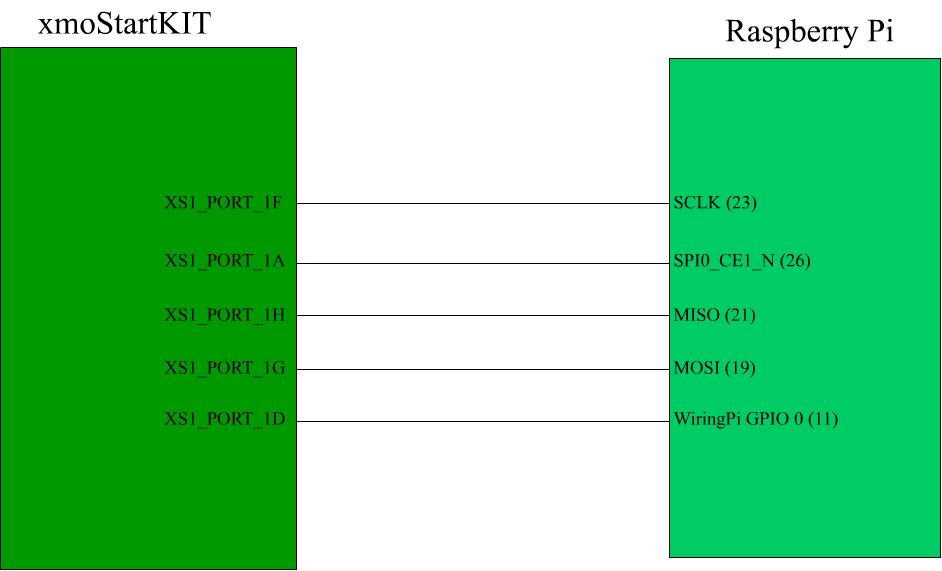
\includegraphics[scale=0.34]{./top.png}
\caption{Conexiones.}
\label{fig:top}
\end{figure}\newpage
\section{Implementación}
La forma en la que se implementaron las rutinas para enviar desde la XMOS a la Rpi de forma ordenada fue la siguiente:
\begin{itemize}
\item Primero se interrumpe la Rpi desde la XMOS.
\item Luego se envía un byte con el tamaño de los datos.
  \item Finalmente se envían los datos con el tamaño ya recibido.
\end{itemize}
Esta forma se debe a que las rutinas de la libreria WiringPi trabajan con la cantidad de bytes enviados, no así la librería de la XMOS.
\begin{figure}[ht!]\centering
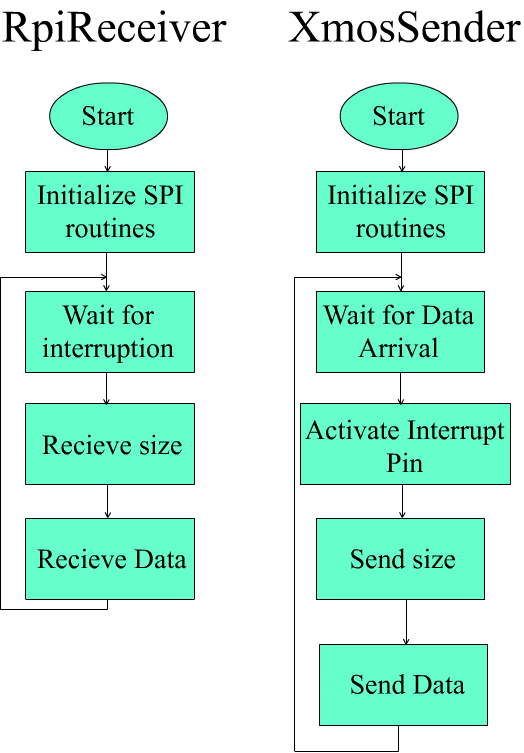
\includegraphics[scale=0.34]{./diag.png}
\caption{Diagrama de flujo, XMOS sender, Rpi receiver.}
\label{fig:top}
\end{figure}
Con respecto al envío desde la Rpi, es mas transparente, pues es el maestro el que inicia la comunicación y se modificó el ejemplo de [3], para recibir datos en la XMOS por SPI como esclavo.\newpage
\section{Repositorio}
El código de las rutinas se encuentra en https://github.com/gopimn/xmosRpiSenderReceiver bajo licencia GPL 3.0, y se compone de dos directorios:
\subsection{src}
En esta capeta se encuentran los {\it headers} para poder usar las diferentes rutinas:
\begin{itemize}
\item {\it rpiReceiver.h},para recibir con la Rpi, contiene la función rpiReceiver, que recibe como argumento el vector de {\it unsigned char} donde guardaremos la data y retorna la cantidad de bytes recibidos.
\item {\it rpiSender.h}, para enviar con la Rpi, contiene la Task rpiSend, que recibe como argumento el vector de {\it unsigned char} donde tenemos la información a enviar y la cantidad de bytes que se quiere enviar, retorna la cantidad de bytes exitosamente enviados.
\item {\it xmosReceiver}, para recibir con la XMOS, contiene la función spiSender, que tiene como argumentos la interfaz SPI(esclavo) y la interfaz {\it receiverSPI\_if}para recibir datos de esta rutina definida en el mismo header, permite crear una Task para llamar a la función xmosRecieve, que ejecuta la adquisición de datos como cliente (revisar documentación [], para más información acerca de los conceptos de interfaz y channend de lenguaje xc).
\item {\it xmosSender.h}, para enviar con la XMOS, contiene la Task spiSender, que tiene como argumentos la interfaz de comunicacion SPI (esclavo), la interfaz {\it senderSPI\_if} y el puerto (GPIO) con el cuál interrumpimos a la Rpi. Esta interfaz permite usar como cliente la función xmosSend, que tiene como argumentos el vector de datos y la cantidad de bytes a enviar.
\end{itemize}
  \subsection{examples}
  En esta carpeta se encuentran los dos ejemplos para ambas aplicaciones, enviar desde la XMOS y recibir desde la XMOS, recordar colocar en el mismo directorio del codigo fuente el header correspondiente definido en el encabezado de cada archivo en esta carpeta.\newpage

%----------------------------------------------------------------------------------------
%	BIBLIOGRAPHY
%----------------------------------------------------------------------------------------
\section{Notas Finales}
\begin{itemize}
\item Es importante conocer los conceptos de interfaz cliente y servidor usados en [1].
\item Existe una inconsistencia con la rutina de la Rpi al tratar de recibir mas de 15 Bytes (ocurre un corrimiento) dada la pobre calidad del reloj del Rpi. Para contrarrestar este efecto, se debe usar la rutina con 10 bytes o menos y llamarla varias veces en caso de tener mucha data, con intervalos de 1 [ms].
\item Es importante tener instalada la librería wiring Pi en la Rpi.
\item Es importante importar en el makefile de la XMOS a las librerias spi y debug\_printf.
\item Recordar colocar los header en la misma carpeta donde se ejecuta los codigos de ejemplo.
  \item En la Rpi compilar con g++ y ejecutar como superusuario.
  \end{itemize}
\section{Bibliografía}
Link en el número.
\begin{itemize}
\item\href{https://www.google.com/url?sa=t&rct=j&q=&esrc=s&source=web&cd=2&cad=rja&uact=8&ved=0ahUKEwjwqO3awdHTAhWDEpAKHURlDr8QFggrMAE&url=https%3A%2F%2Fwww.xmos.com%2Fdownload%2Fprivate%2FXMOS-Programming-Guide-(documentation)(E).pdf&usg=AFQjCNEo1fItwfoJAkXCRro7vJsQjMuLLQ&sig2=PuG2SJMDRsxElWmgEYTTyg}{[1]} XMOS programing guide.
\item\href{https://www.google.com/url?sa=t&rct=j&q=&esrc=s&source=web&cd=2&cad=rja&uact=8&ved=0ahUKEwip7sXCwtHTAhWDDpAKHR1EBkYQFgguMAE&url=https%3A%2F%2Fwww.xmos.com%2Fdownload%2Fprivate%2FstartKIT-Hardware-Manual%25281.0%2529.pdf&usg=AFQjCNFX6eY8WwRSqBPBgmR2k5FZZ1n9zw&sig2=uiL-EIwlkLmJBVE9CTpltQ}{[2]} XMOSSTARTKIT hardware manual.
\item\href{https://www.google.com/url?sa=t&rct=j&q=&esrc=s&source=web&cd=3&cad=rja&uact=8&ved=0ahUKEwjcjpXPwtHTAhUBIpAKHXZuC_cQFggwMAI&url=https%3A%2F%2Fwww.xmos.com%2Fdownload%2Fprivate%2FXMOS-xSOFTip-SPI-Slave-Component-(documentation)(1.3.1rc1.a).pdf&usg=AFQjCNFsuUmAHxuceyPbnxXnlDEBVuXtzw&sig2=obcpHkq4W8-zkXGWF2t1zA}{[3]} XMOS spi slave documentation.
\item\href{http://wiringpi.com/reference/}{[4]} Libreria Wiring pi.
  \end{itemize}

%----------------------------------------------------------------------------------------


\end{document}
